\documentclass[aspectratio=43, t]{beamer}
\usetheme{CSCS}

\usepackage{fontspec}
\usepackage{pgfpages}
\usepackage{minted}
\usepackage{xurl}
\usepackage{hyperref}
\usepackage{booktabs}
\usepackage{multicol}
\usepackage{pgfplots}
\usepackage{tikzpagenodes}
\usetikzlibrary{arrows.meta}

\setminted{autogobble, obeytabs, tabsize=2}
\setsansfont[Scale = 0.85]{TeX Gyre Heros}
\pgfplotsset{
	height = 8cm,
	compat = newest,
	results/.style = {
		xbar,
		xmin = 0,
		xmax = 20,
		ytick = data,
		nodes near coords,
		nodes near coords align = horizontal,
		every axis plot post/.append style = {
			cscsred,
		},
		xticklabel style = {
			/pgf/number format/assume math mode = true,
			font = \sffamily,
		},
		yticklabel style = {
			font = \footnotesize,
			align = right,
			text width = 3cm,
			execute at begin node = \setlength{\baselineskip}{7pt},
		},
		node near coords style = {
			/pgf/number format/assume math mode = true,
			font = \sffamily,
		},
	},
}

% define footer text
\newcommand{\footlinetext}{Rust Webinar}

% Select the image for the title page
%\newcommand{\picturetitle}{cscs_images/image3.pdf}
\newcommand{\picturetitle}{cscs_images/image5.pdf}
%\newcommand{\picturetitle}{cscs_images/image6.pdf}

\author{Michal Sudwoj}
\title{An Overview of Rust}
\subtitle{Webinar}
\date{26.06.2020}

\setbeameroption{show notes on second screen = right}
\begin{document}
% disable Pygment error highlighting
\renewcommand{\fcolorbox}[4][]{#4}

\begin{frame}[plain, c]
	\titlepage
\end{frame}

\section*{Introduction}

\begin{frame}
	\frametitle{Questions}

	\includegraphics[width = \textwidth, height = \textheight, keepaspectratio]{rustacean-flat-gesture}
	\note[item]{Ferris the Crab}
	\note[item]{Use Zoom Q\&A feature, or use the "Raise pincer" button}
\end{frame}

\subsection*{What is Rust?}
\begin{frame}
	\frametitle{\subsecname}

	\begin{itemize}
		\item 2006: personal project of Graydon Hoare
		\item 2010: announced by Mozilla Research
		\item 2015: v1.0
		\item 2016\textendash{}2020: "most loved programming language"
		\item 6 week release cycle
	\end{itemize}
	\note[item]{Used in Firefox (Servo engine), Redox OS}
	\note[item]{Sponsored by Microsoft, Mozilla, Amazon, Google}
	\note[item]{Ferrous Systems GmBH: Sealed Rust - Rust in Safety Critical Domain}

	\vspace{0pt plus 1filll}

	\begin{flushright}
		\includegraphics[width = 5cm, height = 5cm, keepaspectratio]{rust-logo-512x512-blk}
	\end{flushright}

	\vspace*{1cm}
\end{frame}

\subsection*{Installation}
\begin{frame}[fragile]
	\frametitle{\subsecname}

	Using \mintinline{bash}{spack}:
	\begin{minted}{bash}
		$ spack install rust         # for stable
		$ spack install rust@1.43.1  # for v1.43.1
		$ spack install rust@nightly # for nightly
	\end{minted}

	Using \mintinline{bash}{rustup}:
	\begin{minted}{bash}
		$ curl https://sh.rustup.rs -sSf | sh
		$ rustup toolchain install stable  # for stable
		$ rustup toolchain install 1.43.1  # for v1.43.1
		$ rustup toolchain install nightly # for nightly
		$ rustup toolchain install nightly-2020-05-31

		$ rustup default <toolchain>

		$ rustup target install nvptx64-nvidia-cuda
	\end{minted}
	\note[item]{\texttt{cd <project-dir>; rustup override set <toolchain>}}
	\note[item]{\texttt{rustup target install nvptx64-nvidia-cuda}}
\end{frame}

\subsection*{Hello, World!}
\begin{frame}[fragile]
	\frametitle{\subsecname}

	\begin{minted}{bash}
		$ cargo new --bin hello_world
		$ cd hello_world
		$ cat src/main.rs
	\end{minted}
	\note[item]{\texttt{cargo new --bin} for example binary}
	\note[item]{\texttt{cargo new --lib} for example library}
	\note[item]{\texttt{cargo +nightly} for version change}

	\begin{minted}{rust}
		fn main() {
		    println!("Hello, World!");
		}
	\end{minted}

	\begin{minted}{bash}
		$ cargo run
		Hello, World!
	\end{minted}
\end{frame}

\subsection*{Features}
\begin{frame}[fragile]
	\frametitle{\subsecname}

	\begin{itemize}
		\item \texttt{C++}-like syntax
		\item non-mutable and private by default
		\item \mintinline{rust}{struct}s (incl.\ tuple structs)
		\item \mintinline{rust}{enum}s (tagged unions)
		\item \mintinline{rust}{trait}s
		\item \mintinline{rust}{mod}ules
		\item \mintinline{rust}{Iterator}s (think \texttt{C++} ranges / Python for-loops)
		\item UTF-8 support
		\item generics
		\item \textbf{hygenic} macros
		\item attributes incl.\ \mintinline{rust}{#[derive(...)]}
			\note[item]{\mintinline{rust}{cfg} attributes for architectures/os/...}
			\note[item]{\mintinline{rust}{repr} for different \mintinline{rust}{struct} and \mintinline{rust}{enum} representations}
		\item \mintinline{rust}{Result<T, E>} instead of exceptions
		\item \texttt{rustc} LLVM backend
	\end{itemize}
\end{frame}

\subsection*{Standard Library}
\begin{frame}[fragile]
	\frametitle{\subsecname}

	\begin{itemize}
		\item
			\mintinline{rust}{Option<T>}, \note[item]{eg. \mintinline{rust}{Option} optimized for references (null pointer = \mintinline{rust}{None})}
			\mintinline{rust}{Result<T, E>}
		\item Collections:
			\mintinline{rust}{Vec<T>},
			\mintinline{rust}{VecDeque<T>},
			\mintinline{rust}{LinkedList<T>},
			\mintinline{rust}{HashMap<K, V>},
			\mintinline{rust}{BTreeMap<K, V>},
			\mintinline{rust}{HashSet<T>},
			\mintinline{rust}{BTreeSet<T>},
			\mintinline{rust}{BinaryHeap<T>}
		\item Interior mutability: \note[item]{Interior Mutatbility: mutable via \mintinline{rust}{&T}, runtime borrow checking, \mintinline{rust}{!Sync}}
			\mintinline{rust}{Cell<T>},
			\mintinline{rust}{RefCell<T>}
		\item
			\mintinline{rust}{Rc<T>}
		\item Syncronization:
			\mintinline{rust}{Arc<T>},
			\mintinline{rust}{Mutex<T>},
			\mintinline{rust}{RwLock<T>},
			\mintinline{rust}{Barrier},
			\mintinline{rust}{CondVar},
			\mintinline{rust}{mpsc::{Sender, SyncSender, Receiver}}
		\item Traits:
			\mintinline{rust}{Copy},
			\mintinline{rust}{Clone},
			\mintinline{rust}{PartialEq},
			\mintinline{rust}{Eq},
			\mintinline{rust}{PartialOrd},
			\mintinline{rust}{Ord},
			\mintinline{rust}{Display},
			\mintinline{rust}{Debug},
			\mintinline{rust}{Send}, \note[item]{\mintinline{rust}{Send}: type not sendable to another thread}
			\mintinline{rust}{Sync} \note[item]{\mintinline{rust}{Sync}: not shareable between thread (\mintinline{rust}{&T: !Send})}
		\item Intrinsics:
			\mintinline{rust}{core::arch::x86_64::{_mm256_fmadd_pd, ...}}
		\item Assmebly:
			\mintinline{rust}{asm!},
			\mintinline{rust}{global_asm!},
			\mintinline{rust}{llvm_asm!}
	\end{itemize}
\end{frame}

\section*{The Good}
\subsection*{\texorpdfstring{\texttt{cargo}}{cargo}}
\begin{frame}[fragile]
	\frametitle{\secname: \subsecname}

	\begin{minted}[fontsize = \small]{bash}
		$ cargo build [--release | ...]
		$ cargo run [--examples | ... ]
		$ cargo test
		$ cargo bench
		$ cargo doc
		$ cargo fix    # automatically fix errors
		$ cargo fmt    # format code
		$ cargo clippy # lint
		# extensible
		$ cargo mpirun
		$ cargo expand [my_mod::foo]
		$ cargo asm [my_mod::foo]
		$ cargo flamegraph
		$ cargo valgrind
		$ cargo bloat
		# ...
	\end{minted}
	\note[item]{critcmp \url{https://github.com/BurntSushi/critcmp}}
	\note[item]{cargo-benchcmp \url{https://github.com/BurntSushi/cargo-benchcmp}}
	\begin{tikzpicture}[
		remember picture,
		overlay,
		shift = {(current page.south east)}
	]
		\node[anchor = south east, yshift = 1cm] {
			
\includegraphics[width = 6.5cm]{clippy}
		};
	\end{tikzpicture}
\end{frame}

\subsection*{\texorpdfstring{\texttt{build.rs}}{build.rs}}
\begin{frame}
	\frametitle{\secname: \subsecname}

	\begin{itemize}
		\item custom build script (written in Rust!)
		\item crates to call \mintinline{bash}{cc}, \mintinline{bash}{cmake}, generate C bindings (\texttt{bindgen})
		\item compile-time embedding and environment access
	\end{itemize}

	Demo: \url{https://git.cscs.ch/msudwoj/rust-in-hpc/-/tree/master/interop/rust2cpp}
\end{frame}

\subsection*{Ecosystem}
\begin{frame}
	\frametitle{\secname: \subsecname}

	\begin{itemize}
		\item \url{crates.io}
			\begin{itemize}
				\item package registry
				\item custom registries
			\end{itemize}
		\item \url{docs.rs}
	\end{itemize}
	\note[item]{Properly semversion'ed}
	\note[item]{commit \texttt{Cargo.lock} to freeze dependencies}
	\note[item]{high quality packages}
	\note[item]{some used in \texttt{rustc}}
	\note[item]{Supports multiple crate versions in the same program/library}
	\note[item]{Cargo.toml}
	\note[item]{patches, overrides, …}
	\note[item]{build profiles, eg. build dependencies always in release mode}

	\vspace{0pt plus 1filll}

	\begin{flushright}
		\includegraphics[width = 6cm, height = 6cm, keepaspectratio]{Cargo-Logo-Small}
	\end{flushright}
\end{frame}

\begin{frame}
	\frametitle{\secname: \subsecname}

	\begin{multicols}{2}
		\begin{itemize}
			\item \texttt{ndarray}
			\item \texttt{blas}, \texttt{cblas}, \texttt{lapack}, \texttt{lapacke}, \texttt{netlib-src}, \texttt{openblas-src}, \texttt{intel-mkl-src}
			\item \texttt{num}
			\item \texttt{lazy\_static}
			\item \texttt{serde}
			\item \texttt{rayon}, \texttt{crossbeam}, \texttt{parking\_lot}
			\item \texttt{rand}
			\item \texttt{libc}
			\item \texttt{bitflags}
			\item \texttt{proc-macro2}, \texttt{syn}, \texttt{quote}
			\item \texttt{hdf5}
			\item \texttt{mpi}
			\item \texttt{smallvec}
			\item \texttt{tokio}, \texttt{async-std}
			\item \texttt{reqwest}
			\item \texttt{criterion}, \texttt{bencher}
			\item \texttt{thiserror}, \texttt{anyhow}
		\end{itemize}
	\end{multicols}
\end{frame}

\subsection*{Borrow Checker}
\begin{frame}[fragile]
	\frametitle{\secname: \subsecname}

	\begin{minted}{bash}
		$ cat src/main.rs
	\end{minted}
	\begin{minted}{rust}
		fn foo<T>(x: T, y: &T, z: &mut T) {}
		fn main() {
		  let mut s = String::from("Hello, World!");
		  foo(s, &s, &mut s);
		}
	\end{minted}
	\begin{minted}{bash}
		$ cargo build
	\end{minted}
\end{frame}

\begin{frame}[fragile]
	\frametitle{\secname: \subsecname}

	\begin{minted}[fontsize = \scriptsize]{bash}
		error[E0382]: borrow of moved value: `s`
		 --> src/main.rs:7:12
		6 |     let mut s = String::from("Hello, World!");
		  |         ----- move occurs because `s` has type `std::string::String`,
		                  which does not implement the `Copy` trait
		7 |     foo(s, &s, &mut s);
		  |         -  ^^ value borrowed here after move
		  |         |
		  |         value moved here
		error[E0502]: cannot borrow `s` as mutable because it is also borrowed
		              as immutable
		 --> src/main.rs:7:16
		7 |     foo(s, &s, &mut s);
		  |     ---    --  ^^^^^^ mutable borrow occurs here
		  |     |      |
		  |     |      immutable borrow occurs here
		  |     immutable borrow later used by call
		error: aborting due to 2 previous errors
		Some errors have detailed explanations: E0382, E0502.
		For more information about an error, try `rustc --explain E0382`.
		error: could not compile `foo`.
		To learn more, run the command again with --verbose.
	\end{minted}
	\note[item]{Spans}
	\note[item]{\mintinline{bash}{rustc --explain EXXXX}}
\end{frame}

\subsection*{String printing and formatting}
\begin{frame}[fragile]
	\frametitle{\secname: \subsecname}

	\begin{minted}{bash}
		$ cat src/main.rs
	\end{minted}
	\begin{minted}{rust}
		fn main() {
		  let e = std::env::VarError::NotPresent;
		  println!("Display: {}", e);
		  println!("Debug:   {:?}", e);
		}
	\end{minted}
	\begin{minted}{bash}
		$ cargo run
		Display: environment variable not found
		Debug:   NotPresent
	\end{minted}

	On your own types:
	\begin{minted}{rust}
		#[derive(Debug)]
		struct Foo { /* ... */ }
		impl std::fmt::Display for Foo { /* ... */ }
	\end{minted}
\end{frame}

\subsection*{Pattern matching}
\begin{frame}[fragile]
	\frametitle{\secname: \subsecname}

	\begin{minted}{rust}
		use std::num::NonZeroU8;
		use rand::random;
		let x = NonZeroU8::new(random::<u8>());
		if let Some(x) = x {
			match x {
				1       => print!("x = 1"),
				2..10   => print!("2 <= x < 10"),
				10..=20 => print!("10 <= x <= 20"),
				_       => print!("20 < x"),
			}
		}
	\end{minted}
	\note[item]{Also: guards, bindings (\texttt{@})}
\end{frame}

\subsection*{\texorpdfstring{\texttt{unsafe}}{unsafe}}
\begin{frame}
	\frametitle{\secname: \subsecname}

	Superpowers:
	\begin{itemize}
		\item Dereference a raw pointer
		\item Call an unsafe function or Method
		\item Access or mutate a mutable static variable
		\item Implement an unsafe trait
		\item Access fields of \mintinline{rust}{union}s
	\end{itemize}
	\textbf{Thats it. Nothing else.}
	\note{
		In particular, some things are still UB:
		\begin{itemize}
			\item data races
			\item dereferencing dangling or unaligned pointers
			\item uninitialized memory (use \mintinline{rust}{std::mem::MaybeUninit<T>})
			\item \textellipsis
		\end{itemize}
		see \url{https://doc.rust-lang.org/reference/behavior-considered-undefined.html}

		Inversely, things that are still safe, but generally undesireable:
		\begin{itemize}
			\item deadlocks
			\item memory leaks
			\item exiting without calling destructors
			\item integer overflow
		\end{itemize}
		see \url{https://doc.rust-lang.org/reference/behavior-not-considered-unsafe.html}
	}
\end{frame}

\subsection*{Macros [sic!]}
\begin{frame}[fragile]
	\frametitle{\secname: \subsecname}

	\begin{minted}[fontsize=\footnotesize]{rust}
		#[macro_export]
		macro_rules! assert {
		  ($cond: expr) => {
		    assert!($cond, "\nassertion failed: {}", stringify!($expr))
		  };
		  ($cond: expr,) => { assert!($cond) };
		  ($cond: expr, $($arg: tt)+) => {
		    if !expr {
		      let msg = $crate::format!($($arg)*);
		      unsafe {
		          ::core::arch::nvptx::__assert_fail(
		          msg.as_ptr(), file!().as_ptr(),
		          line!(), "".as_ptr()
		        )
		      }
		    }
		  };
		}
	\end{minted}
	\note[item]{"macros-by-example"}
	\note[item]{hygenic}
	\note[item]{on syntactic level (token trees)}
\end{frame}

\subsection*{\texorpdfstring{\texttt{proc\_macro}s}{proc\_macros}}
\begin{frame}[fragile]
	\frametitle{\secname: \subsecname}

	\begin{minted}[fontsize = \small]{rust}
		#[proc_macro_attribute]
		pub fn shared(_attr: TokenStream, var: TokenStream)
			-> TokenStream {
			let stmt = parse_macro_input!(var as Stmt);
			let (ident, ty,) = parse_local(&stmt);
			let result = quote! {
				struct Shared<T> { /* ... */ }
				let mut #ident: Shared<#ty> = Shared::new();
			};
			result.into()
		}

		// usage
		pub unsafe extern "ptx-kernel" fn foo( /* ... */ ) {
			#[shared]
			let mut s: [f32; 3];
			// -> let mut s: Shared<[f32; 3]> = Shared::new();
		}
	\end{minted}

	\note[item]{Rust function that transforms the \texttt{TokenStream} at compile time}
	\note[item]{DSLs! Especially using eg. \texttt{combine\_proc\_macro}}
\end{frame}

\subsection{\texorpdfstring{\texttt{async/.await}}{async/.await}}
\begin{frame}[fragile]
	\frametitle{\secname: \subsecname}

	\begin{minted}{rust}
		async fn foo() -> Result<u8> { /* ... */ }

		#[tokio::main]
		async fn main() {
			let future_foo = foo();   // nothing happens: lazy!
			let x = future_foo.await; // evaluate now!
		}
	\end{minted}
	\note[item]{\mintinline{rust}{Future}s in rust are lazy!}
	\note[item]{They get evaluated only upon being \mintinline{rust}{.await}ed}
	\note[item]{Zero-cost}
	\note[item]{Requires executor}
\end{frame}

\section*{The Bad(?)}
\subsection*{Function overloading}
\begin{frame}[fragile]
	\frametitle{\secname: \subsecname}

	\begin{minted}[fontsize = \footnotesize]{rust}
		impl String {
			pub fn new() -> Self { /* ... */ }
			pub fn with_capacity(capacity: usize) -> Self { /* ... */ }
			pub fn from_raw_parts(
			  buf: *mut u8, length: usize, capacity: usize
			) -> Self { /* ... */ }
			pub fn from_utf8(vec: Vec<u8>)
			  -> Result<Self, FromUtf8Error> { /* ... */ }
			pub fn from_utf8_unchecked(bytes: Vec<u8>)
			  -> Self { /* ... */ }
			pub fn from_utf8_lossy(v: &[u8]) -> Cow<str> { /* ... */ }
			pub fn from_utf16(v: &[u16])
			  -> Result<Self, FromUtf16Error> { /* ... */ }
			pub fn from_utf16_lossy(v: &[u16]) -> Self { /* ... */ }
		}
		impl From<&'_ String>   for String { /* ... */ }
		impl From<&'_ str>      for String { /* ... */ }
		impl From<Box<str>>     for String { /* ... */ }
		impl From<Cow<'a, str>> for String { /* ... */ }
		// ...
	\end{minted}
	\note[item]{By design choice}
	\note[item]{\url{https://internals.rust-lang.org/t/justification-for-rust-not-supporting-function-overloading-directly/7012}}
	\note[item]{Can be alleviated by traits, but is considered an anti-pattern (other than eg.\ From)}
\end{frame}

\subsection*{Inheritance}
\begin{frame}[fragile]
	\frametitle{\secname: \subsecname}

	\begin{multicols}{2}
		Composition
		\begin{minted}[fontsize = \small]{rust}
			struct Foo { /* ... */ }
			impl Foo {
			  pub fn bar(&self) {
			    /* ... */
			  }
			}
			struct Baz {
			  foo: Foo,
			  /* ... */
			}
			impl Baz {
			  pub fn bar(&self) {
			    self.foo.bar()
			  }
			}
		\end{minted}
		\columnbreak
		Traits
		\begin{minted}[fontsize = \small]{rust}
			struct Foo { /* ... */ }
			struct Baz { /* ... */ }
			trait Barable {
			  pub fn bar(&self);
			}
			impl Barable for Foo {
			  fn bar(&self) { /* ... */ }
			}
			impl Barable for Baz {
			  fn bar(&self) { /* ... */ }
			}
		\end{minted}
	\end{multicols}
	\note[item]{Can also do blanket implementation in Barable}
\end{frame}

\subsection*{Unstable features}
\begin{frame}[fragile]
	\frametitle{\secname: \subsecname}

	\begin{itemize}
		\item \mintinline{rust}{#![feature(const_generics)]}
		\item \mintinline{rust}{#![feature(specialization)]}
		\item \mintinline{rust}{#![feature(const_fn)]}
		\item \mintinline{rust}{#![feature(fn_traits, unboxed_closures)]}
	\end{itemize}
\end{frame}

\subsection*{Tier 3 CUDA support}
\begin{frame}
	\frametitle{\secname: \subsecname}

	As of May 15th 2020: Tier 2!

	Works, but \textellipsis
	\begin{itemize}
		\item (only on nightly)
		\item lots of boilerplate
		\item \mintinline{rust}{unsafe} / unsound
		\item can still call (C++) CUDA functions using FFI
	\end{itemize}
	\note[item]{"Hacky": requires \texttt{ptx-linker}, which fixes link issues}
	\note[item]{rustc is unaware of CUDA threading model -> cannot use slices/borrowck in CUDA device code}
	\note[item]{No support for \mintinline{cuda}{__shared__} or \mintinline{cuda}{__const__}}
	\note[item]{Tier 1: guaranteed to work (automated testing): currently i686 and x68\_64}
	\note[item]{Tier 2: guaranteed to build: a lot}
	\note[item]{Tier 3: preliminary support}
\end{frame}

\section*{The Ugly}
\subsection*{A Web of \texorpdfstring{\mintinline{rust}{String}}{String}s}
\begin{frame}[c]
	\frametitle{\secname: \subsecname}

	\centering
	\begin{tabular}{l l l l}
		\toprule
		Type  & Owned                       & Slice                    & \\
		\midrule
		UTF-8 & \mintinline{rust}{String}   & \mintinline{rust}{str}   & UTF-8 (incl. \texttt{\textbackslash{}0}), not NUL-terminated \\
		C     & \mintinline{rust}{CString}  & \mintinline{rust}{CStr}  & \mintinline{c}{char}/\mintinline{c}{wchar_t}, NUL-terminated \\
		OS    & \mintinline{rust}{OsString} & \mintinline{rust}{OsStr} & OS default encoded \\
		Path  & \mintinline{rust}{PathBuf}  & \mintinline{rust}{Path}  & this wrapper around \mintinline{rust}{OsString}/\mintinline{rust}{OsStr} \\
		Bytes & \mintinline{rust}{Vec<u8>}  & \mintinline{rust}{[u8]}  & \\
		\bottomrule
	\end{tabular}

	\vfill

	\begin{description}
		\item[\mintinline{rust}{char}:] 1\textendash{}4 byte UTF-8 scalar value
		\item[\mintinline{rust}{u8}:] byte
	\end{description}
\end{frame}

\section*{Conclusion}
\begin{frame}
	\frametitle{\secname}

	Rust…
	\begin{itemize}
		\item … takes getting used to
		\item … has great tooling
		\item … in still missing some crucial features (on stable)
			\begin{itemize}
				\item const generics
				\item specialization
			\end{itemize}
		\item … has zero-cost abstractions
		\item … has good interop with C (and other languages)
		\item … helps you avoid memory errors
		\item … makes shared memory parallelism hard
	\end{itemize}
\end{frame}

\begin{frame}
	\frametitle{Questions?}

	\includegraphics[width = \textwidth, height = \textheight, keepaspectratio]{rustacean-flat-gesture}
\end{frame}

\begin{frame}
	\frametitle{Hit me up!}

	\begin{itemize}
		\item \url{https://git.cscs.ch/msudwoj/rust-in-hpc}
		\item Slack: \texttt{@Michal Sudwoj}
		\item Email: \texttt{\href{mailto:msudwoj@student.ethz.ch}{msudwoj@student.ethz.ch}}
	\end{itemize}
\end{frame}

\cscsthankyou{Thank you for your attention.}

\section*{References}
\begin{frame}
	\frametitle{\secname}

	\begin{itemize}
		\item The Rust Programming Language: \url{https://doc.rust-lang.org/book/title-page.html}
		\item The Rustonomicon: \url{https://doc.rust-lang.org/nomicon/index.html}
		\item The Cargo Book: \url{https://doc.rust-lang.org/cargo/index.html}
		\item Rust Forge: \url{https://forge.rust-lang.org/index.html}
	\end{itemize}
\end{frame}

\section*{Extras}
\subsection*{\texorpdfstring{\texttt{rustc}}{rustc} compilation process}
\begin{frame}[fragile]
	\frametitle{\subsecname}

	\begin{itemize}
		\item crate: translation unit
		\item codegen-unit: LLVM module
		\item incremental compilation: cache intermediate results
		\item \hyperref[https://github.com/mozilla/sccache]{\texttt{sccache}}: cache between workspaces
		\item \mintinline{rust}{#[inline]}: enable inlining across crate boundaries
	\end{itemize}
	\note[item]{codegen-unit allows parallel compilation}
	\note[item]{incremental compilation caches intermediate results and only recompiles if necessary}

	\centering
	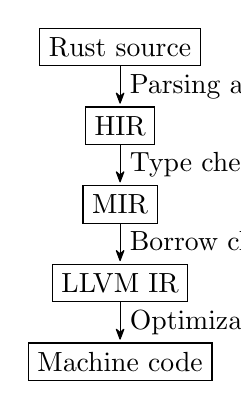
\begin{tikzpicture}
		\begin{scope}[
			every node/.style = {
				draw,
				shape = rectangle
			}
		]
			\node (source)                      {Rust source};
			\node (hir)     [below of = source] {HIR};
			\node (mir)     [below of = hir]    {MIR};
			\node (llvm)    [below of = mir]    {LLVM IR};
			\node (machine) [below of = llvm]   {Machine code};
		\end{scope}

		\begin{scope}[
			every node/.style = {auto},
			shorten > = 1pt,
			> = {Stealth[round]}
		]
			\draw [->] (source) to node {\rlap{Parsing and desugaring}}        (hir);
			\draw [->] (hir)    to node {\rlap{Type checking}}                 (mir);
			\draw [->] (mir)    to node {\rlap{Borrow checking, optimization}} (llvm);
			\draw [->] (llvm)   to node {\rlap{Optimization}}                  (machine);
		\end{scope}
	\end{tikzpicture}
	\par
\end{frame}

\section*{Questionnaire Results}
\subsection*{What is your experience with…}
\subsubsection*{C++?}
\begin{frame}[fragile]
	\frametitle{\subsecname{} \subsubsecname}

	\begin{tikzpicture}
		\begin{axis}[
			results,
			symbolic y coords = {
				{It's equivalent to \texttt{C += 1}},
				{I did an online tutorial},
				{I did a small project},
				{I use it daily},
				{I helped design it}
			}
		]
			\addplot coordinates {
				( 1,{I helped design it})
				(17,{I use it daily})
				( 1,{I did a small project})
				( 0,{I did an online tutorial})
				( 0,{It's equivalent to \texttt{C += 1}})
			};
		\end{axis}
	\end{tikzpicture}
\end{frame}

\subsubsection*{Fortran?}
\begin{frame}[fragile]
	\frametitle{\subsecname{} \subsubsecname}

	\begin{tikzpicture}
		\begin{axis}[
			results,
			symbolic y coords = {
				{I was hoping it would die out before I had to learn it},
				{I did an online tutorial},
				{I did a small project},
				{I use it daily},
				{I helped design it}
			}
		]
			\addplot coordinates {
				( 1,{I helped design it})
				( 2,{I use it daily})
				( 5,{I did a small project})
				( 1,{I did an online tutorial})
				(10,{I was hoping it would die out before I had to learn it})
			};
		\end{axis}
	\end{tikzpicture}
\end{frame}

\subsubsection*{Haskell?}
\begin{frame}[fragile]
	\frametitle{\subsecname{} \subsubsecname}

	\begin{tikzpicture}
		\begin{axis}[
			results,
			symbolic y coords = {
				{I've haven't been too eager to learn about monads},
				{I did an online tutorial},
				{I did a small project},
				{I use it daily},
				{I helped design it}
			}
		]
			\addplot coordinates {
				( 0,{I helped design it})
				( 0,{I use it daily})
				( 3,{I did a small project})
				( 5,{I did an online tutorial})
				(11,{I've haven't been too eager to learn about monads})
			};
		\end{axis}
	\end{tikzpicture}
\end{frame}

\subsubsection*{Rust?}
\begin{frame}[fragile]
	\frametitle{\subsecname{} \subsubsecname}

	\begin{tikzpicture}
		\begin{axis}[
			results,
			symbolic y coords = {
				{It's oxidized iron, brown and coarse to the touch},
				{I did an online tutorial},
				{I did a small project},
				{I use it daily},
				{I helped design it}
			}
		]
			\addplot coordinates {
				( 0,{I helped design it})
				( 0,{I use it daily})
				( 2,{I did a small project})
				( 2,{I did an online tutorial})
				(15,{It's oxidized iron, brown and coarse to the touch})
			};
		\end{axis}
	\end{tikzpicture}
\end{frame}

\subsection*{These days…}
\begin{frame}[fragile]
	\frametitle{\subsecname}

	\begin{tikzpicture}
		\begin{axis}[
			results,
			symbolic y coords = {
				{I write a lot of CUDA},
				{I make heavy use of type generics},
				{I design and implement DSLs},
				{I make heavy use of compile time programming},
				{I spend way too much time fighting the build system},
			}
		]
			\addplot coordinates {
				(14,{I spend way too much time fighting the build system})
				(11,{I make heavy use of compile time programming})
				( 9,{I design and implement DSLs})
				( 8,{I make heavy use of type generics})
				( 8,{I write a lot of CUDA})
			};
		\end{axis}
	\end{tikzpicture}
\end{frame}

\begin{frame}[fragile]
	\frametitle{\subsecname}

	\begin{tikzpicture}
		\begin{axis}[
			results,
			symbolic y coords = {
				{I write a lot of (asynchronous) task-based routines},
				{I try not to slack while my code is compiling},
				{I write complex object-oriented code, with lots of inheritance},
				{I write a lot of MPI code},
				{I try do decipher what the compiler is trying to tell me},
			}
		]
			\addplot coordinates {
				( 7,{I try do decipher what the compiler is trying to tell me})
				( 7,{I write a lot of MPI code})
				( 7,{I write complex object-oriented code, with lots of inheritance})
				( 5,{I try not to slack while my code is compiling})
				( 5,{I write a lot of (asynchronous) task-based routines})
			};
		\end{axis}
	\end{tikzpicture}
\end{frame}

\begin{frame}[fragile]
	\frametitle{\subsecname}

	\begin{tikzpicture}
		\begin{axis}[
			results,
			symbolic y coords = {
				{I sprinkle OpenACC directives everywhere},
				{I sprinkle OpenMP directives everywhere},
				{I try to drop to BLAS as soon as possible},
				{I mostly write glue code, and interface between different programming languages},
				{I write highly optimized kernels with using intrinsics and/or assembly},
			}
		]
			\addplot coordinates {
				( 5,{I write highly optimized kernels with using intrinsics and/or assembly})
				( 4,{I mostly write glue code, and interface between different programming languages})
				( 4,{I try to drop to BLAS as soon as possible})
				( 3,{I sprinkle OpenMP directives everywhere})
				( 0,{I sprinkle OpenACC directives everywhere})
			};
		\end{axis}
	\end{tikzpicture}
\end{frame}

\subsection*{Most bugs I encounter…}
\begin{frame}[fragile]
	\frametitle{\subsecname}

	\begin{tikzpicture}
		\begin{axis}[
			results,
			symbolic y coords = {
				{are in other people's code},
				{involve dangling references or pointers},
				{are out-of-bound errors or off-by-one errors},
				{are performance regressions},
				{involve race conditions},
			}
		]
			\addplot coordinates {
				(12,{involve race conditions})
				(10,{are performance regressions})
				( 4,{are out-of-bound errors or off-by-one errors})
				( 3,{involve dangling references or pointers})
				( 2,{are in other people's code})
			};
		\end{axis}
	\end{tikzpicture}

	Other: typos
\end{frame}

\subsection*{In the webinar, I would like to see…}
\begin{frame}[fragile]
	\frametitle{\subsecname}

	\begin{tikzpicture}
		\begin{axis}[
			results,
			symbolic y coords = {
				{how to interface Rust with Fortran},
				{how Rust compiler errors look like},
				{how the this thing called the "borrow checker" works},
				{how to interface Rust with Python},
				{how Rust manages dependencies},
				{how inheritance works in Rust},
				{how to write low-level code in Rust},
				{how macros can be not-evil},
				{how to interface Rust with C/C++},
			}
		]
			\addplot coordinates {
				(12,{how to interface Rust with C/C++})
				(10,{how macros can be not-evil})
				(10,{how to write low-level code in Rust})
				( 9,{how inheritance works in Rust})
				( 9,{how Rust manages dependencies})
				( 7,{how to interface Rust with Python})
				( 5,{how the this thing called the "borrow checker" works})
				( 3,{how Rust compiler errors look like})
				( 2,{how to interface Rust with Fortran})
			};
		\end{axis}
	\end{tikzpicture}
\end{frame}

\end{document}
